\subsection{What Constitutes Reception?}
\begin{frame}[t]{What Constitutes Reception?}
\small
\begin{block}{}
\textsl{Reception} happens when one planet (A) is in the domicile or exaltation of another planet (B) whom it aspects or conjuncts. The aspect (or conjunction) from planet \textsl{A} must \textsl{perfect} (become exact)  before planet \textsl{B} moves into another sign or a third planet (C) intercedes by completing its own aspect or conjunction with planet \textsl{B}.
\end{block}

While Masha'allah appears to have been the first to begin categorizing and explaining the way reception, applications, and separations indicate outcomes Sahl ibn Bishr al-Israili (786-845) seems to have been the first to spell out the 16 distinct modes of the "perfection and destruction of things". These were also listed and amplified by  Abu Ma'shar (787-886),  and Ibn Ezra (1089-1164).

Examples from these authors are used to name and describe the various ways in which reception can occur. The referenced texts are:
\begin{itemize}
\small
\item \textsl{The Introduction to the Science of the Judgments of the Stars} by Sahl ibn Bishr trans. James Holden, AFA, 2008 
\item \textsl{The Astrology of Sahl B. Bishr Vol. I} trans. Ben Dykes, Cazimi Press, 2019

\item \textsl{The Abbreviation of the Introduction to Astrology} by Abu Ma'shar trans. Charles Burnett, ARHAT, 2nd. printing, 2000

\item \textsl{Ibn Ezra: The Beginning of Wisdom} trans. Meira Epstein, ARHAT, 1998
\end{itemize}

\end{frame}
% -------------------------------------------------------------------
\subsubsection{Perfect Reception - Pusing Nature}
\begin{frame}[t]{What Constitutes Reception - Perfect Reception: Pushing Nature}
\small
\vspace{0.1cm}
\begin{columns}[T, onlytextwidth]
\column{0.5\textwidth}
An example of \textbf{perfect reception} is a planet (A) applying to the domicile or exaltation ruler (B) of the sign it occupies.\footnotemark[1] Ibn Ezra (p121) says the ruler (B) "will confer its nature upon" planet A, and "there will be joy in the matter'', but other authors say A pushes B's nature onto B.  \\
\vspace{0.2cm}
\textbf{Example (A $\Rightarrow$ B): \Moon\ in \Aries\ $\Rightarrow$ \Mars\ or \Sun} 
\ul
\vspace{0.2cm}
\Moon\ in \Aries\ applying to either of \\
\Mars\ (domicile ruler of \Aries) or \\
\Sun\ (exaltation ruler of \Aries) \\
\vspace{0.2cm}
\Mars\ or the \Sun\ can be in any sign; they receive the \Moon, accepting her disposition, because she is in \Aries\ which \Mars\ rules by domicile and the \Sun\ by exaltation. \\
\column{0.5\textwidth}

\begin{center}
{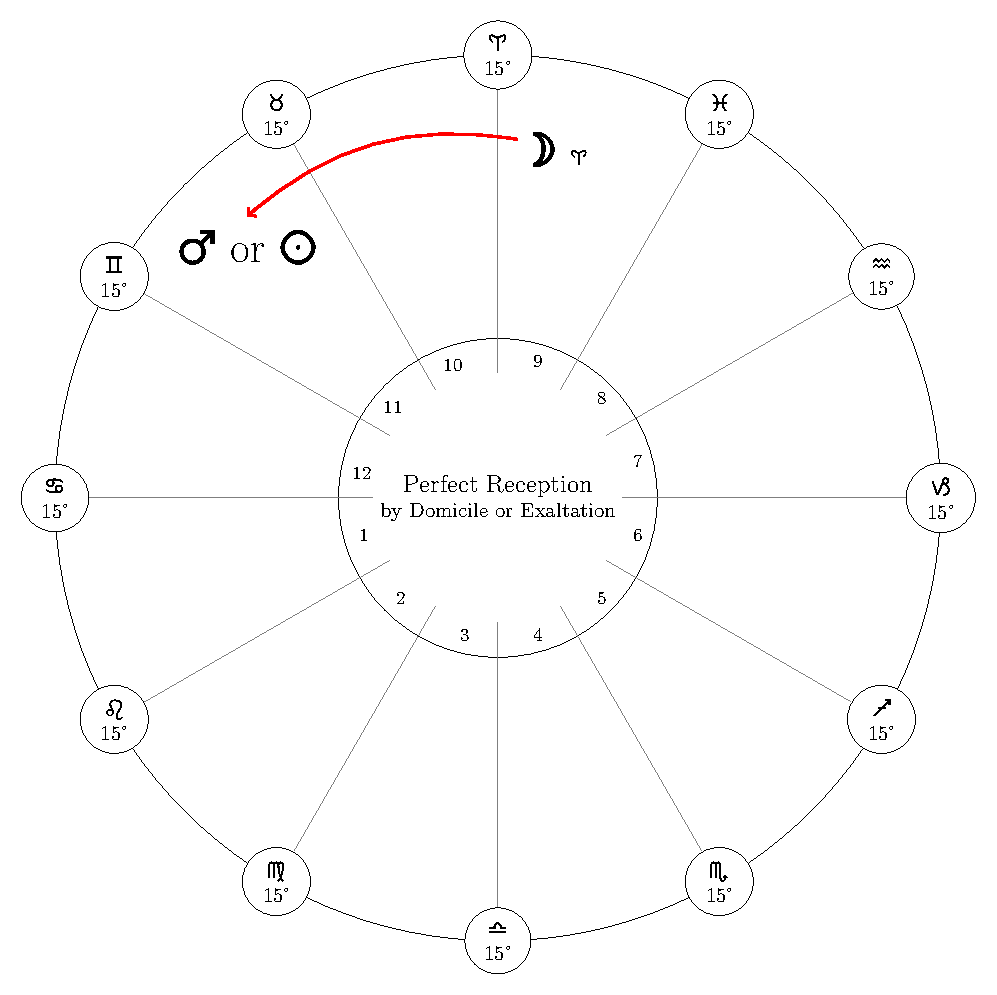
\includegraphics[width=0.8\textwidth]{charts/01-perfect-reception}} \\
\end{center}

\end{columns}
\vspace{0.2cm}
\footnotetext[1]{Sahl, p.18}
\end{frame}
% ----------------------------------------------------
\subsubsection{A Weaker Reception - Pushing Power}
\begin{frame}[t]{What Constitutes Reception - A Weaker Reception: Pushing Power}
\footnotesize
\begin{columns}[T, onlytextwidth]
\column{0.5\textwidth}
A weaker reception occurs when a planet in its own domicile or exaltation, applying to another planet, pushes its own power  to the other planet (Abu Ma'shar). Ibn Ezra calls it \textsl{"conferring influence"}; Sahl, \textsl{"giving virtue" or "committing disposition"}.\footnotemark[1] Here, \textsl{A} gives his own authority and resources to \textsl{B} and "the matter will be perfected as desired." \\
\vspace{0.2cm}
\textbf{Example (A $\Rightarrow$ B):} \Mars\ or \Sun\ in \Aries\ $\Rightarrow$  \Saturn \\
\ul
\vspace{0.2cm}
\Mars\ or \Sun\ in \Aries\ applying to  \\
\Saturn\ in any sign

\vspace{0.25cm}
\Mars\ or the \Sun\ are gving their disposition (virtue, power) to \Saturn.

\vspace{0.25cm}
\textbf{Note:} that strictly speaking Sahl would consider this a 'non-reception' as \Aries\ is \Saturn's Fall.\footnotemark[2] Other authors accept it as a corrupted reception.

\column{0.5\textwidth}
\begin{center}
{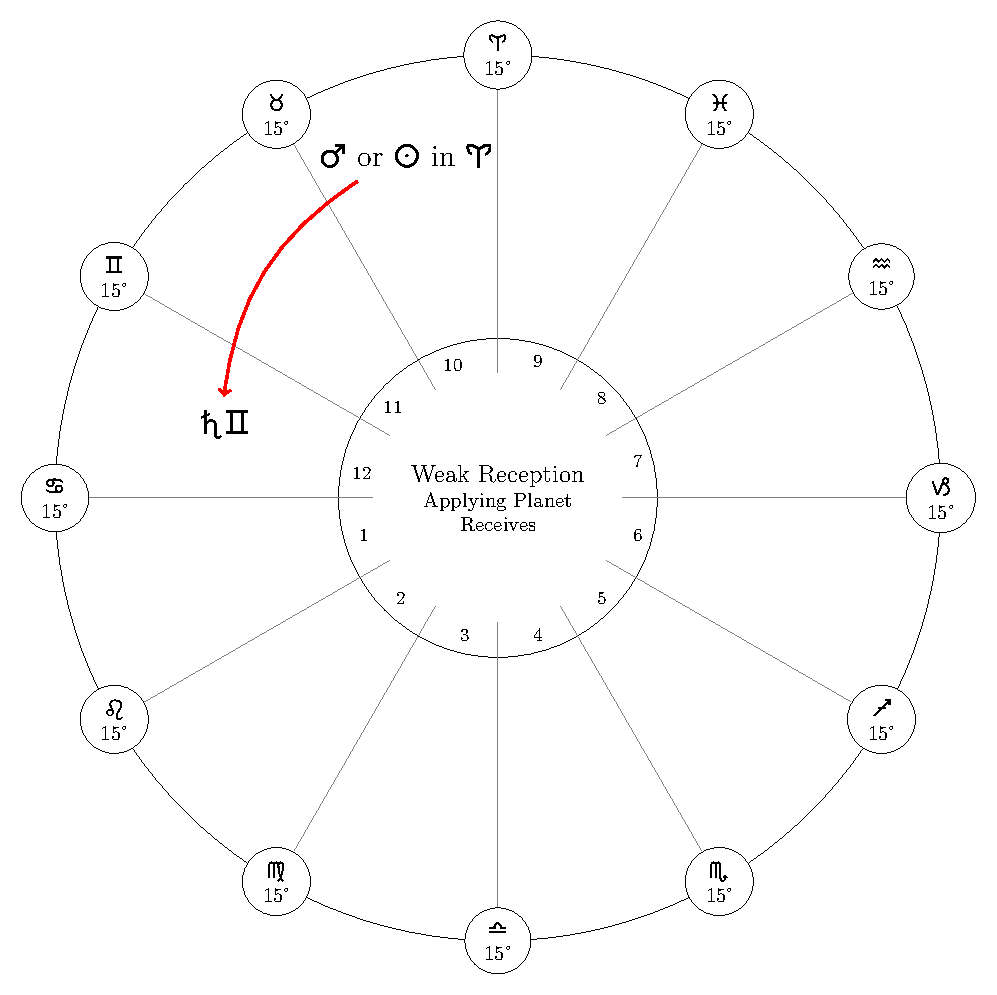
\includegraphics[width=\textwidth]{charts/01-weaker-reception}} \\
\end{center}

\end{columns}
\vspace{0.2cm}
\footnotetext[1]{Abu Ma'shar, p.25;Ibn Ezra, p. 121; Sahl p20 Holden}
\footnotetext[2]{Sahl, Dykes trans. p.62; Holden's, p.19}
\end{frame}
% -------------------------------------------------
\subsubsection{Pushing Two Natures}
\begin{frame}[t]{What Constitutes Reception - Pushing Two Natures}
\begin{columns}[T, onlytextwidth]
\column{0.5\textwidth}
When a planet (A) in its domicile or exaltation applies to another planet (B) who also has dignity in \textsl{A's} place \textsl{A} is said to be "pushing two natures" onto \textsl{B}; his own and \textsl{B}'s.\footnotemark[1]\\
\vspace{0.2cm}
\textbf{Example (A $\Rightarrow$ B):} \Venus\ in \Pisces\ $\Rightarrow$ \Jupiter \\
\ul
\Venus\ exalted in \Pisces\ applies to \\
\Jupiter\ who is the domicile ruler of \Pisces \\
\Venus\ pushes her own and \Jupiter's nature, onto \Jupiter \\
\vspace{0.2cm}

Rob Hand also describes another form of reception called \textbf{communion} which happens when two planets are found in the same sign with one ruling the sign and the other being the exaltation ruler of the sign e.g. \Moon\ and \Jupiter\ both in \Cancer, or \Mars\ and \Sun\ both in \Aries, etc.

\column{0.5\textwidth}
\vspace{-0.5cm}
\begin{center}
{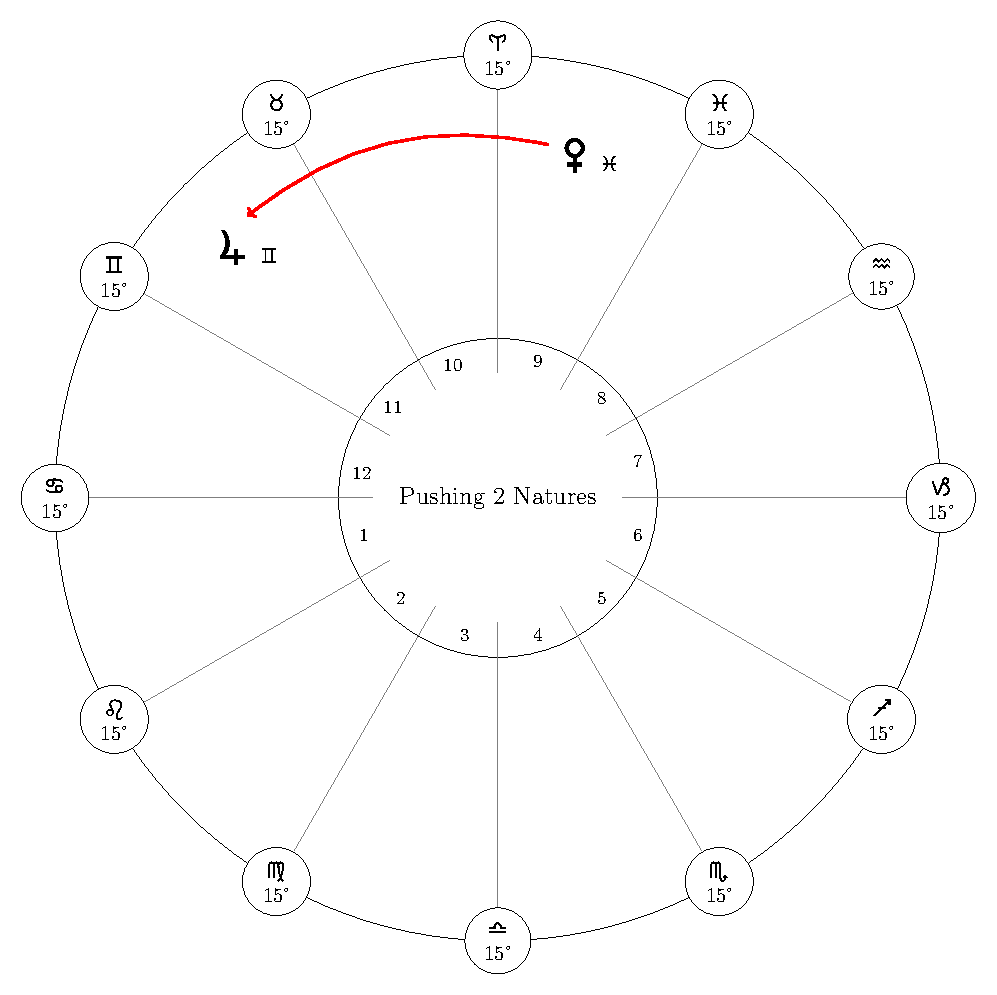
\includegraphics[width=\textwidth]{charts/01-pushing-two-natures}} \\
\end{center}

\end{columns}
\footnotetext[1]{Abu Ma'shar p25; Ibn Ezra p122 calls it \textsl{"conferring of two natures"}}
\end{frame}

% ----------------------------------------------------
\subsubsection{Mutual Reception}
\begin{frame}[t]{What Constitutes Reception - Mutual Reception}
\small
\begin{columns}[T, onlytextwidth]
\column{0.5\textwidth}
\textbf{Example:} \Mars\ 10 \Capricorn\ $\Rightarrow$ \Square\ \Saturn\ 20 \Aries \\
\ul
\vspace{0.25cm}
\Mars\ is in \Saturn's domicile (\Capricorn) applying to \Saturn \\
\Saturn\ is in \Mars's domicile (\Aries), therefore, \\
\Mars\ receives \Saturn\ by domicile, and \\
\Saturn\ receives \Mars\ by domicile \\
\vspace{0.25cm}
\footnotesize
This is  \textbf{Mutual Reception} [MR] by \textsl{domicile} \\
where \Mars\ commits his disposition to \Saturn, who receives it (as \Mars\ is in \Saturn's domicile) and in turn, \Mars\ receives \Saturn's disposition (as \Saturn\ is in \Mars\ domicile); essentially, the two commit to helping each other.\footnotemark[1]

\vspace{0.25cm}
This is the strongest form of reception; the second strongest form occurs when there is mutual reception by \textsl{exaltation}. e.g. both planets are in each other's sign of exaltation. i.e. \Venus\ in \Cancer\ \Trine\ \Jupiter\ in \Pisces.

\column{0.5\textwidth}

\begin{center}
{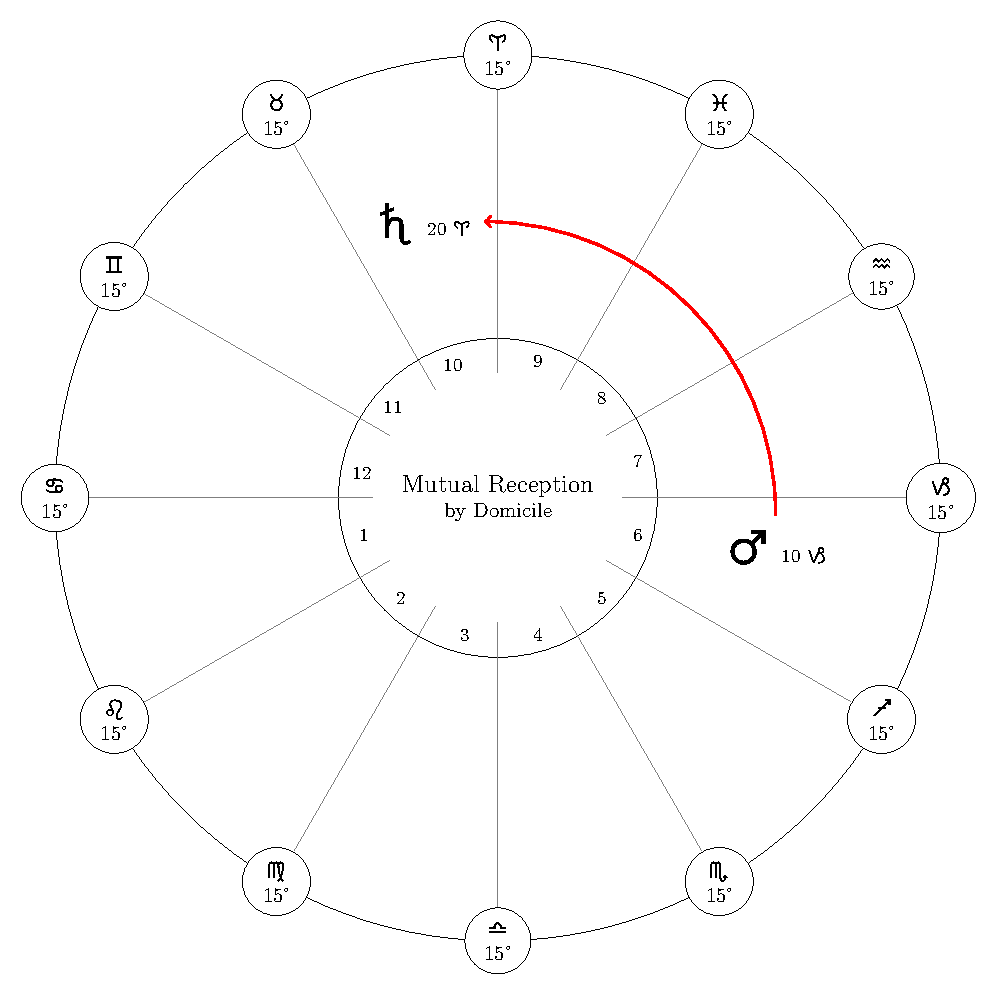
\includegraphics[width=0.9\textwidth]{charts/01-MR-by-domicile}} \\
\end{center}

\end{columns}
\footnotetext[1]{Masha'allah [RH] p3; note that Sahl would call this a non-reception as \Saturn\ is in his Fall.}
\end{frame}
% ---------------------------------------------
\subsubsection{Corrupted Receptions and Returns}
\begin{frame}[t]{What Constitutes Reception - Corrupted Receptions or Returns}
There can be \textbf{no reception} if neither planet has dignity in their own or the other planet's place e.g. \Mercury\ $\Rightarrow$ \Jupiter\ in \Taurus\ where both are peregrine. Although Masha'allah does describe a situation which allows for eventual reception if the applied to planet (\Jupiter\ in this example) goes on to apply, with reception, to a third planet.\\
\vspace{0.25cm}
While Sahl denies reception if a planet is in his own Fall or applying to another planet from that planet's Fall, the other authors appear to accept the reception but say that it is \textbf{corrupted or greatly diminished} i.e. the outcome to the matter is far less than what was hoped for or fails to last.\\
\vspace{0.25cm}
As well, a receiving planet that is \textbf{retrograde} or \textbf{USB} will \textbf{return} what it received, destroying it in the process. The same occurs if both planets are cadent.\footnotemark[1] \\
\vspace{0.25cm}
Still another form of return occurs when a planet applies to a cadent planet, in which case Sahl says the matter \textsl{"will not have an ending"}.

\footnotetext[1]{Sahl [Holden] p20}
\end{frame}
% ----------------------------------------------------
\begin{frame}[t]{What Constitutes Reception Continued}

Masha'allah tells us that if the matter being analyzed has to do with a King, the Exaltation rulers will have more authority over the matter than the domicile rulers.

As a general rule, reception is stronger if the planet applied to (usually the heavier planet) receives the applying planet (usually the lighter planet).

The later authors (Sahl, Abu Ma'shar, Ibn Ezra) also allowed reception by triplicity, term, and face but only considered it to be an \textsl{effective} reception if it involved at least two of these minor dignities i.e. received by triplicity and term or triplicity and face or term and face. Masha'allah does mention these minor dignities in his \textsl{Book of Thoughts and Intentions} but only in relation to determining which planet has the most authority over a specific matter; he does not use them in any of his \textsl{On Reception} examples.\footnotemark[1]
\begin{block}{}
Reception is important as it implies completion; that the matter will be disposed of, effected, by the receiving planet; that what the significator commits to another will be brought into being and realized.
\end{block}
\footnotetext[1]{Although Sahl does claim that Masha'allah allowed reception by the minor dignities [JH p18].}
\end{frame}